
\documentclass[sigconf]{acmart}
\usepackage{caption}
\usepackage{subcaption}
\usepackage{todonotes}
\newcommand{\TODO}[2]{\todo[inline]{#1: #2}}

\setcopyright{none}
\copyrightyear{2022}
\acmYear{2022}
\acmDOI{}

\acmConference[ERN'22]{Accepted at the 2022 Emerging Researchers National (ERN) Conference in STEM}{due to COVID-19, the conference is postponed until 2023}{Washington, D.C.}
\acmBooktitle{Accepted at the 2022 Emerging Researchers National (ERN) Conference in STEM, Washington, D.C., due to COVID-19, the conference is postponed until 2023}
\acmPrice{}
\acmISBN{}
%%\citestyle{acmauthoryear}

\makeatletter
\def\@copyrightspace{\relax}
\makeatother

\begin{document}

\title{Time Series Analysis of Blockchain-Based Cryptocurrency Price Changes}

\author{Jacques Fleischer}
\email{jacques.fleischer002@mymdc.net}
\affiliation{%
  \institution{Miami Dade College}
  \streetaddress{11011 SW 104th St}
  \city{Miami}
  \state{FL}
  \country{USA}
}

\author{Gregor von Laszewski}
\email{laszewski@gmail.com}
\orcid{0000-0001-9558-179X}
\affiliation{%
  \institution{University of Virginia}
  \streetaddress{Biocomplexity Institute\\
                Town Center Four\\
                994 Research Park Boulevard}
  \city{Charlottesville}
  \state{VA}
  \country{USA}
}

\author{Carlos Theran}
\email{carlos.theran@famu.edu}
\affiliation{%
  \institution{Florida A\&M University}
  \streetaddress{1601 S Martin Luther King Jr Blvd}
  \city{Tallahassee}
  \state{FL}
  \country{USA}
}

\author{Yohn Jairo Parra Bautista}
\email{yohn.parrabautista@famu.edu}
\affiliation{%
  \institution{Florida A\&M University}
  \streetaddress{1601 S Martin Luther King Jr Blvd}
  \city{Tallahassee}
  \state{FL}
  \country{USA}
}


\renewcommand{\shortauthors}{J.P. Fleischer, G. von Laszewski, C. Theran, Y. J. Parra Bautista.}

\begin{abstract}
  In this paper we apply neural networks and Artificial Intelligence (AI) to historical records of high-risk cryptocurrency coins to train a prediction model that guesses their price. This paper's code contains Jupyter notebooks, one of which outputs a timeseries graph of any cryptocurrency price once a CSV file of the historical data is inputted into the program. Another Jupyter notebook trains an LSTM, or a long short-term memory model, to predict a cryptocurrency's closing price. The LSTM is fed the close price, which is the price that the currency has at the end of the day, so it can learn from those values. The notebook creates two sets: a training set and a test set to assess the accuracy of the results.

The data is then normalized using manual min-max scaling so that the model does not experience any bias; this also enhances the performance of the model. Then, the model is trained using three layers— an LSTM, dropout, and dense layer—minimizing the loss through 50 epochs of training; from this training, a recurrent neural network (RNN) is produced and fitted to the training set. Additionally, a graph of the loss over each epoch is produced, with the loss minimizing over time. Finally, the notebook plots a line graph of the actual currency price in red and the predicted price in blue. The process is then repeated for several more cryptocurrencies to compare prediction models. The parameters for the LSTM, such as number of epochs and batch size, are tweaked to try and minimize the root mean square error.
\end{abstract}


\begin{CCSXML}
<ccs2012>
 <concept>
  <concept_id>10010405.10003550.10003552</concept_id>
  <concept_desc>Applied computing~E-commerce infrastructure</concept_desc>
  <concept_significance>500</concept_significance>
 </concept>
 <concept>
  <concept_id>10010405.10010481.10010487</concept_id>
  <concept_desc>Applied computing~Forecasting</concept_desc>
  <concept_significance>500</concept_significance>
 </concept>
</ccs2012>
\end{CCSXML}

\ccsdesc[500]{Applied computing~E-commerce infrastructure}
\ccsdesc[500]{Applied computing~Forecasting}

\keywords{blockchain, time series, finance}

\maketitle


\section{Introduction}

Blockchain is {\em an open, distributed ledger} which records transactions of cryptocurrency. Systems in blockchain are decentralized, which means that these transactions are shared and distributed among all participants on the blockchain for maximum accountability. Furthermore, this new blockchain technology is becoming an increasingly popular alternative to mainstream transactions through traditional banks \cite{c2}. These transactions utilize blockchain-based {\em cryptocurrency}, which is a popular investment of today's age, particularly in Bitcoin. However, the U.S. Securities and Exchange Commission warns that high-risk accompanies these investments \cite{c1}. 

Artificial Intelligence (AI) can be used to predict the prices' behavior to avoid cryptocurrency coins' severe volatility that can scare away possible investors \cite{c3}. AI and blockchain technology make an ideal partnership in data science; the insights generated from the former and the secure environment ensured by the latter create a goldmine for valuable information. For example, an up-and-coming innovation is the automatic trading of {\em digital investment assets} by AI, which will hugely outperform trading conducted by humans \cite{c5}. This innovation would not be possible without the construction of a program which can pinpoint the most ideal time to buy and sell. Similarly, AI is applied in this experiment to predict the future price of cryptocurrencies on a number of different blockchains, including the Electro-Optical System and Ethereum. 

Long short-term memory (LSTM) is a neural network (form of AI) which ingests information and processes data using a {\em gradient-based learning algorithm} \cite{c6}. This creates an algorithm that improves with additional parameters; the algorithm {\em learns} as it ingests. LSTM neural networks will be employed to analyze pre-existing price data so that the model can attempt to generate the future price in varying timetables, such as ten days, several months, or a year from the last date. This innovation could provide as a boon for insights into investments with potentially great returns; it could also contribute to a positive cycle of attracting investors to a coin, which results in a price increase, which repeats. The main objective is to provide insights for investors on an up-and-coming product: cryptocurrency.

\section{Datasets}

This paper utilizes yfinance, a Python module which downloads the historical prices of a cryptocurrency from the first day of its inception to whichever day the program is executed. For example, the Yahoo Finance page for EOS-USD is the source for Figure \ref{fig:eos-price} \cite{c4}. Figure \ref{fig:eos-price} shows the historical data on a line graph when the program receives EOS-USD as an input.

\begin{figure}[htb]
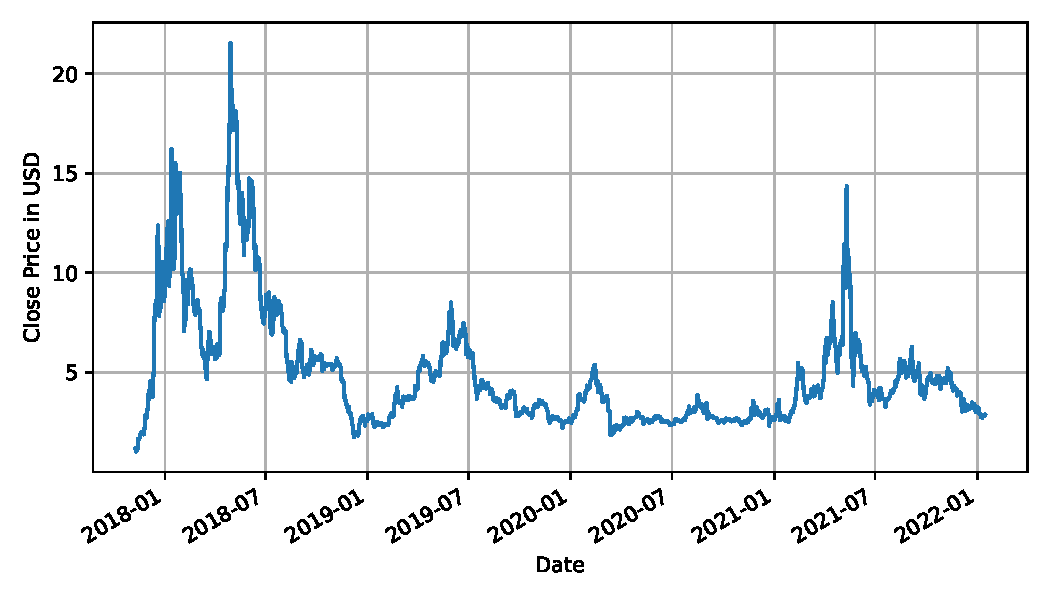
\includegraphics[width=\columnwidth]{images/EOS-USD-price.pdf}
\caption{Line graph of EOS price from 9 November 2017 to 13 January 2022. Generated using yfinance-lstm.ipynb \cite{c13} located in project/code, utilizing price data from Yahoo Finance \cite{c4}.}
\label{fig:eos-price}
\end{figure}

\section{Architecture}

\begin{figure}[htb]
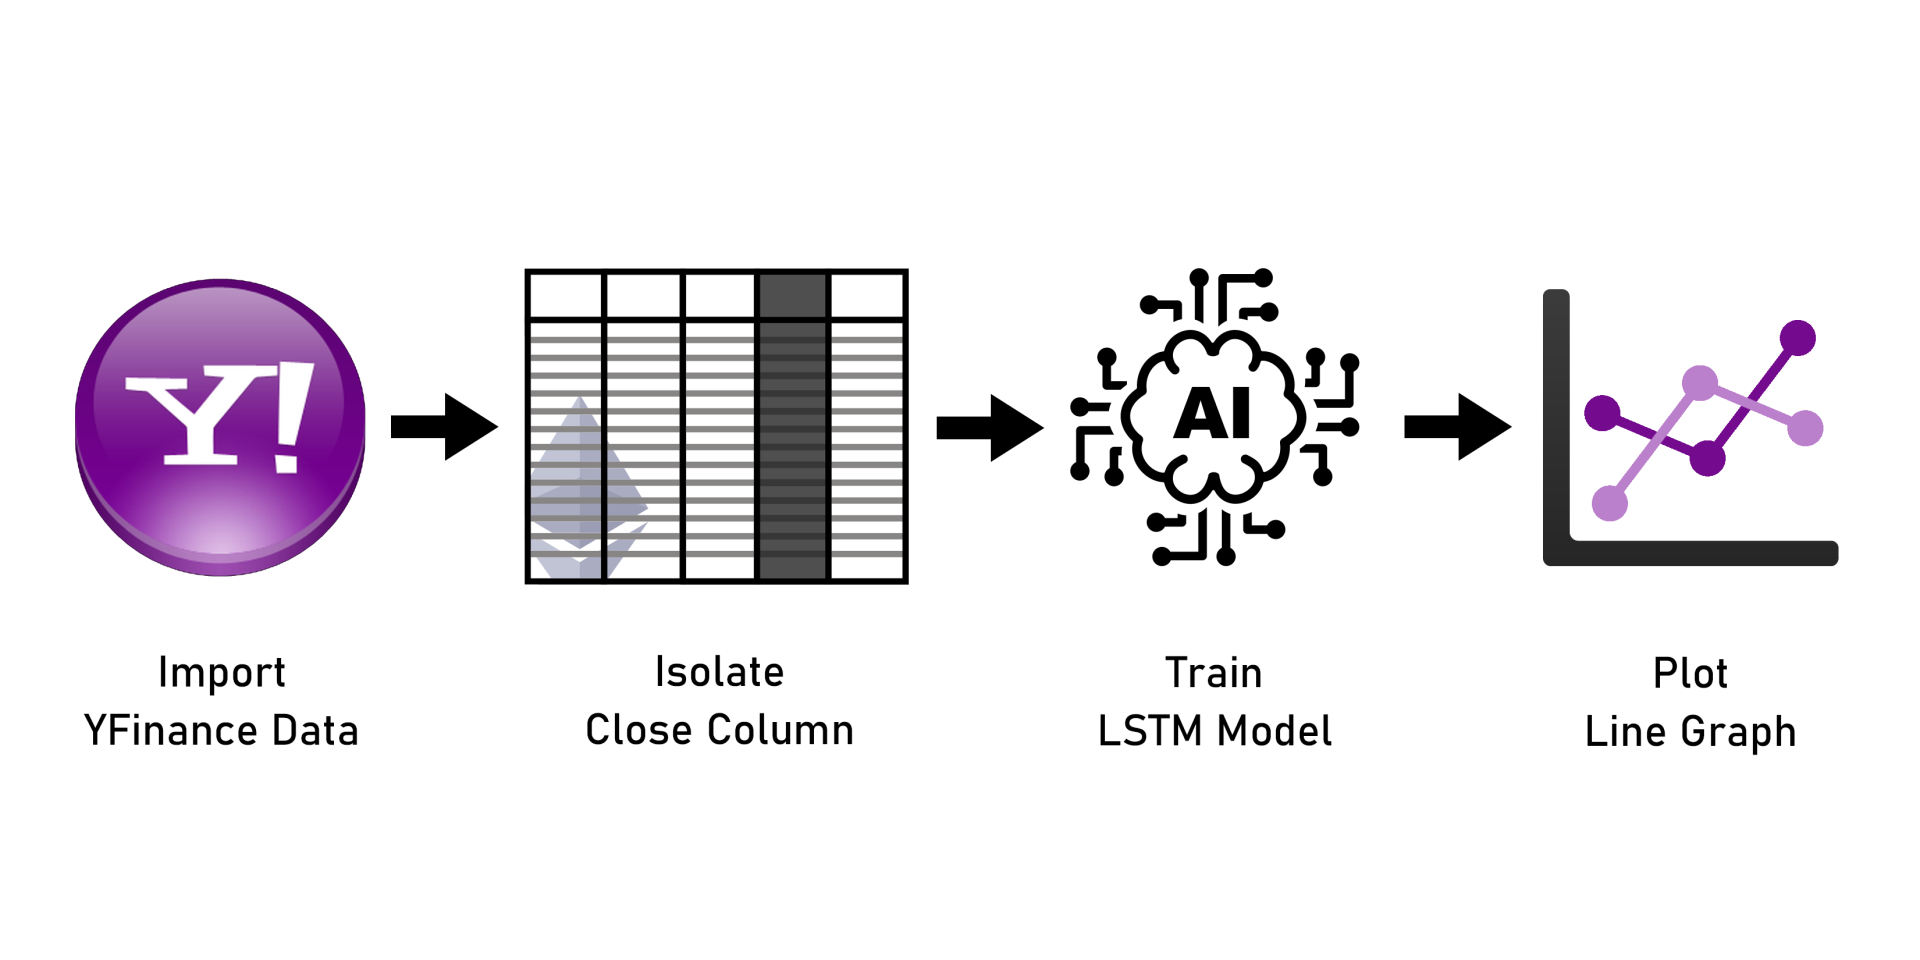
\includegraphics[width=\columnwidth]{images/architecture-process.png}
\caption{The process of producing LSTM timeseries based on cryptocurrency price.}
\label{fig:arch-process}
\end{figure}

This program undergoes the four main phases outlined in Figure \ref{fig:arch-process}, which are: retrieving data from Yahoo Finance \cite{c4}, isolating the Close prices (the price the cryptocurrency has at the end of each day), training the LSTM to predict Close prices, and plotting the prediction model, respectively.

\section{Implementation}

Initially, this program was meant to scrape prices using the BeautifulSoup Python module; however, slight changes in a financial page's website caused the code to break. Alternatively, Kaggle offered historical datasets of cryptocurrency, but they were not up to date. Thus, the final method of retrieving data is from Yahoo Finance through the yfinance Python module, which returns the coins' price from the day to its inception to the present day.

The code is inspired from Towards Data Science articles by Serafeim Loukas \cite{c7} and Viraf \cite{c11}, who explore using LSTM to predict stock timeseries. This program contains adjustments and changes to their code so that cryptocurrency is analyzed instead. We opt to use LSTM (long short-term memory) to predict the price because it has a memory capacity, which is ideal for a timeseries data set analysis such as cryptocurrency price over time. LSTM can remember historical patterns and use them to inform further predictions; it can also selectively choose which datapoints to use and which to disregard for the model \cite{c8}. For example, this experiment's code isolates only the close values to predict them and nothing else.

Firstly, the code asks the user for the ticker of the cryptocurrency that is to be predicted, such as EOS-USD or BTCUSD. A complete list of acceptable inputs is under the Symbol column at the Yahoo Finance list of cryptocurrencies \cite{c17} but theoretically, the program should be able to analyze traditional stocks as well.

Then, the program downloads the historical data for the corresponding coin through the yfinance Python module \cite{c18}. The data must go through normalization for simplicity and optimization of the model. Next, the Close data (the price that the currency has at the end of the day, everyday since the coin's inception) is split into two sets: a training set and a test set, which are further split into their own respective x and y sets to guide the model through training. 

The training model is run through a layer of long short-term memory, as well as a dropout layer to prevent overfitting and a dense layer to give the model a memory capacity. Figure \ref{fig:alstm} showcases the setup of the LSTM layer.

The entire program which performs all of the aforementioned steps can be found on GitHub \cite{c13}.

\begin{figure}[htb]
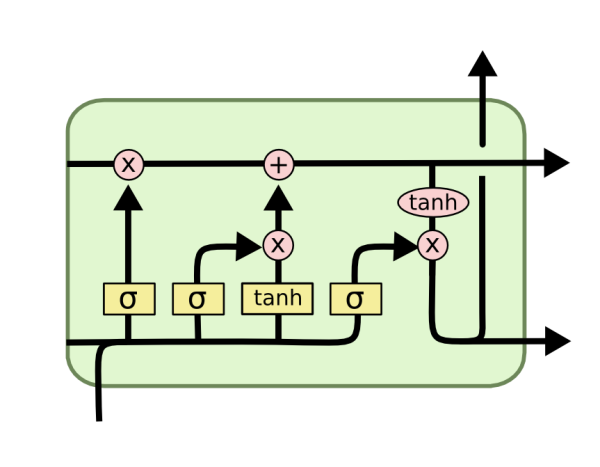
\includegraphics[width=0.5\columnwidth]{images/lstm.png}
\caption{Visual depiction of one layer of long short-term memory \cite{c9}.}
\label{fig:alstm}
\end{figure}

Figures \ref{fig:prediction-model} through \ref{fig:epoch} use the EOS-USD data set from November 9th, 2017 to January 13th, 2022; furthermore, these figures were all produced within the yfinance-lstm Jupyter Notebook \cite{c13}. Within the trained model, only the last 200 days are predicted so that the model can analyze the preexisting data prior to the 200 days for the sake of training.

After training through 50 epochs, the program generated Figure \ref{fig:prediction-model}, a line graph of the prediction model.

\begin{figure}[htb]
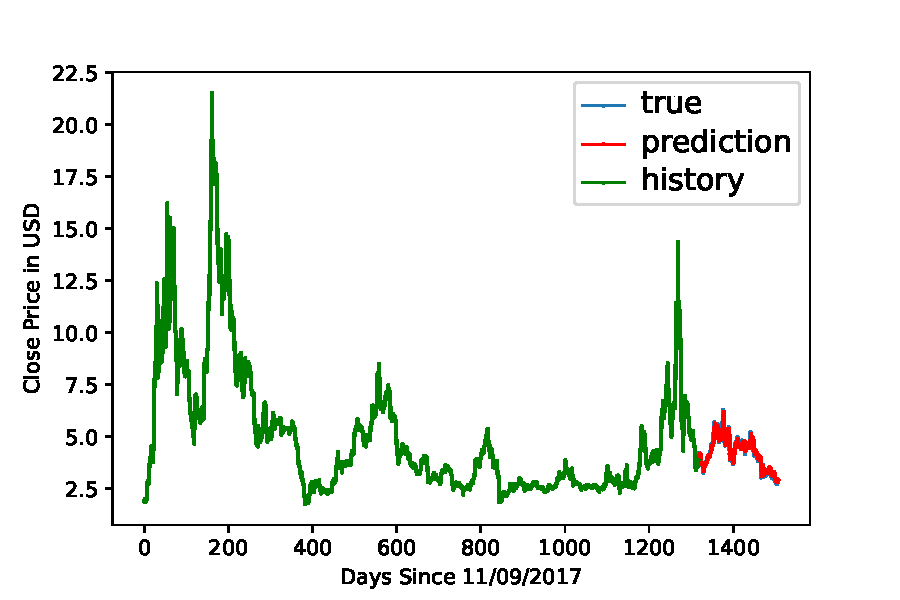
\includegraphics[width=\columnwidth]{images/EOS-USD-prediction-model.pdf}
\caption{EOS-USD price overlayed with the latest 200 days predicted by LSTM.}
\label{fig:prediction-model}
\end{figure}

\begin{figure}[htb]
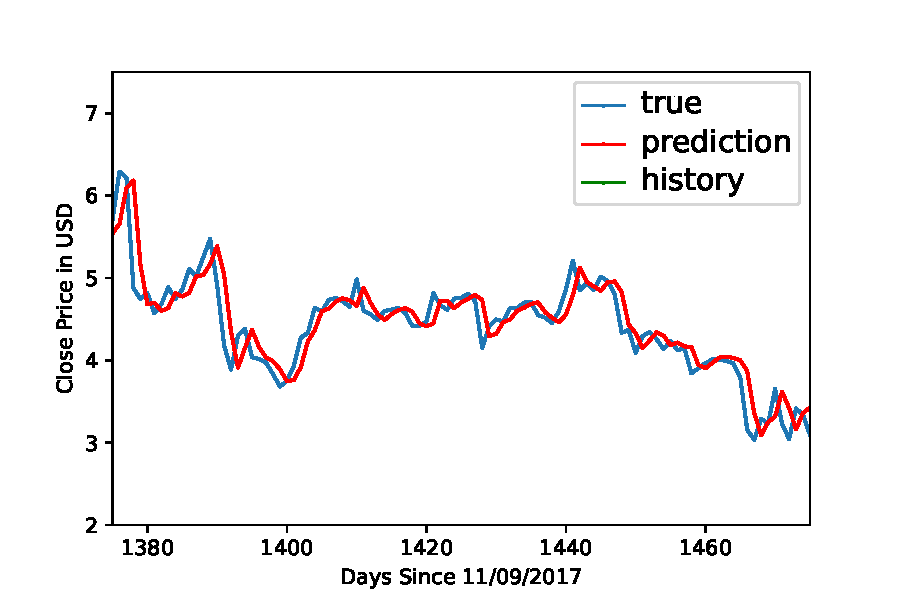
\includegraphics[width=\columnwidth]{images/EOS-USD-prediction-model-zoomed.pdf}

\caption{Zoomed-in graph (same as Figure \ref{fig:prediction-model} but scaled x and y-axis for readability.}
\label{fig:zoomed}
\end{figure}

During training, the number of epochs can affect the model loss. According to Figures \ref{fig:loss} and \ref{fig:epoch}, the loss starts to minimize around the 25th epoch of training. The greater the number of epochs, the sharper and more accurate the prediction becomes, but it does not vastly improve after around the 25th epoch.

\begin{figure}[htb]
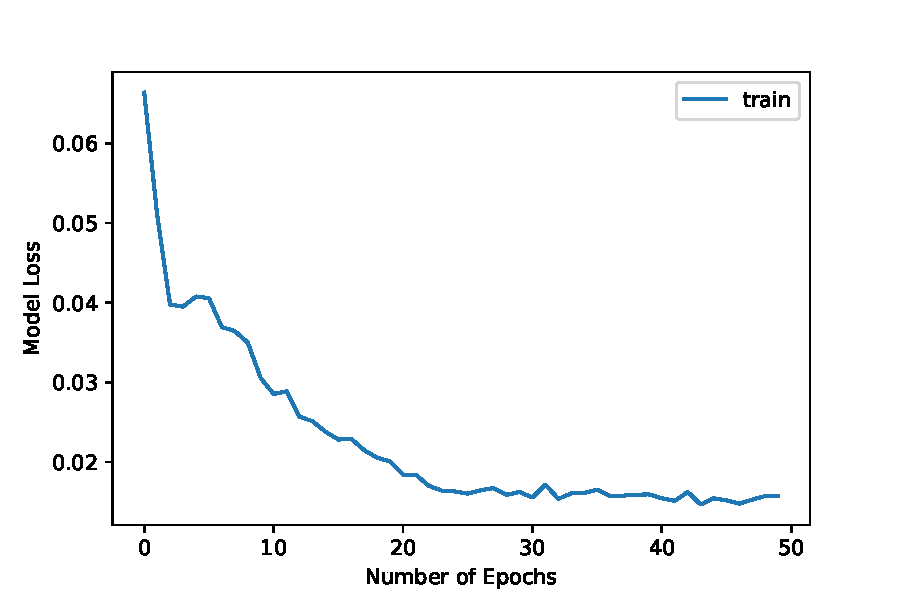
\includegraphics[width=\columnwidth]{images/EOS-USD-training-loss.pdf}

\caption{Line graph of model loss over the number of epochs the prediction model completed using EOS-USD data set.}
\label{fig:loss}
\end{figure}

% \begin{figure*}[htb]
% 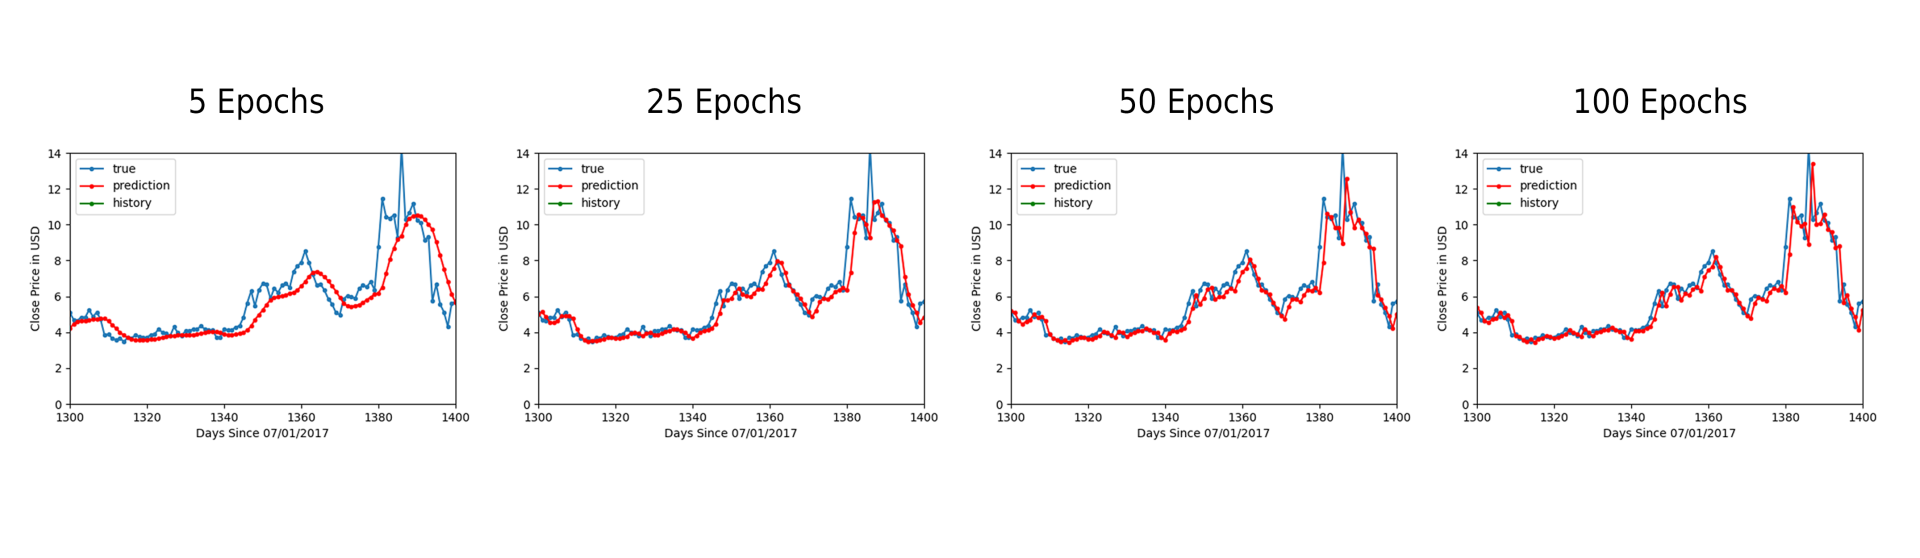
\includegraphics[width=\textwidth]{images/adjusting-epochs.png}
% \vspace{-48pt}
% \caption{Effect of EOS-USD prediction model based on number of epochs completed}
% \label{fig:epoch}
% \end{figure*}


\begin{figure*}[htb]
\centering
     \begin{subfigure}[b]{0.49\textwidth}
         \centering
         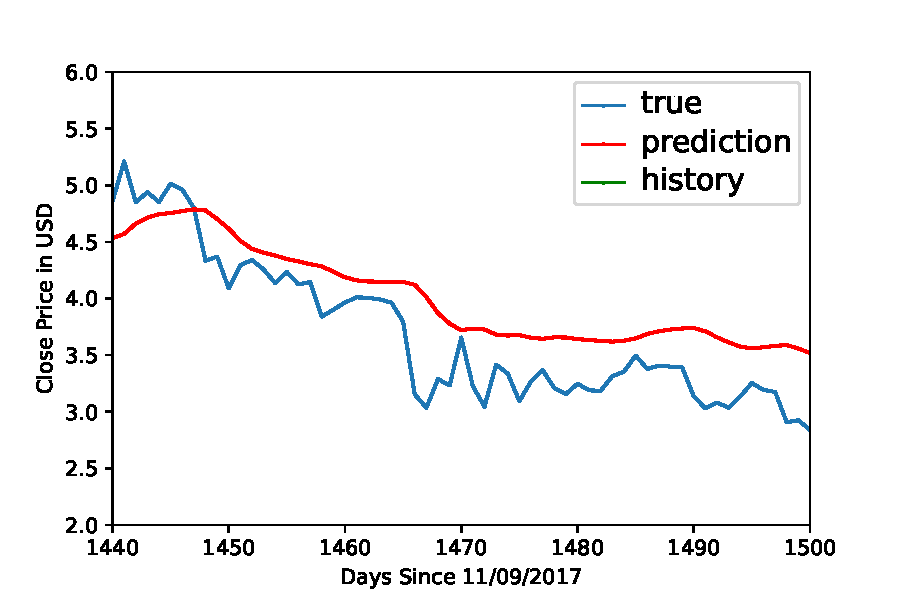
\includegraphics[width=\textwidth]{images/EOS-USD-epoch-5.pdf}
         \caption{5 Epochs}
         \label{fig:epochs-5}
     \end{subfigure}
     \hfill
    \begin{subfigure}[b]{0.49\textwidth}
         \centering
         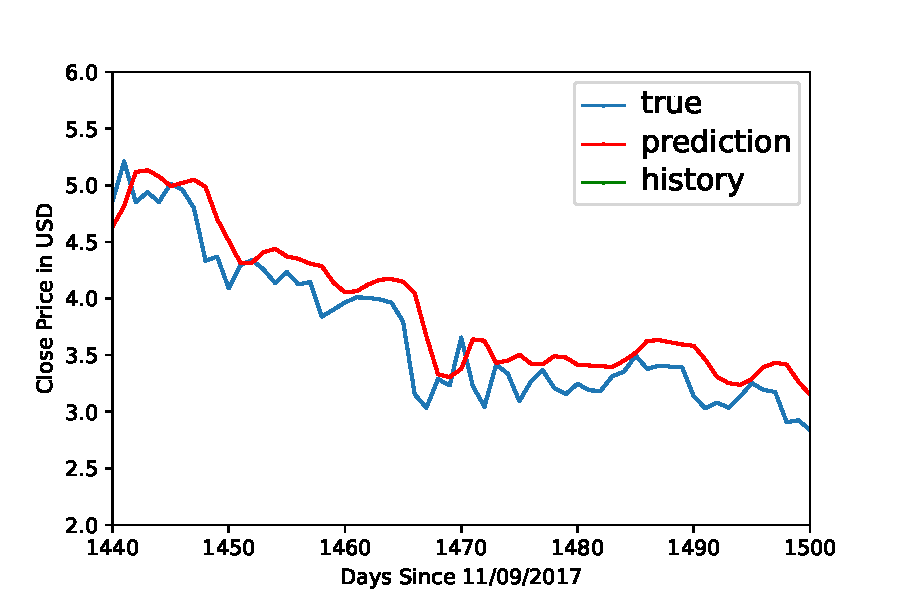
\includegraphics[width=\textwidth]{images/EOS-USD-epoch-25.pdf}
         \caption{25 Epochs}
         \label{fig:epochs-25}
     \end{subfigure}
     \\
     \begin{subfigure}[b]{0.49\textwidth}
         \centering
         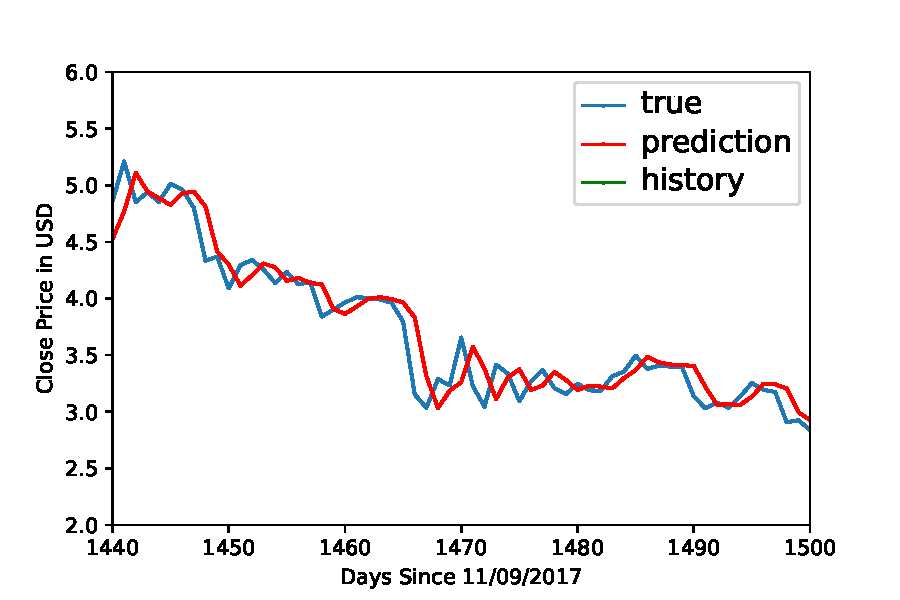
\includegraphics[width=\textwidth]{images/EOS-USD-epoch-50.pdf}
         \caption{50 Epochs}
         \label{fig:epochs-50}
     \end{subfigure}
     \hfill
    \begin{subfigure}[b]{0.49\textwidth}
         \centering
         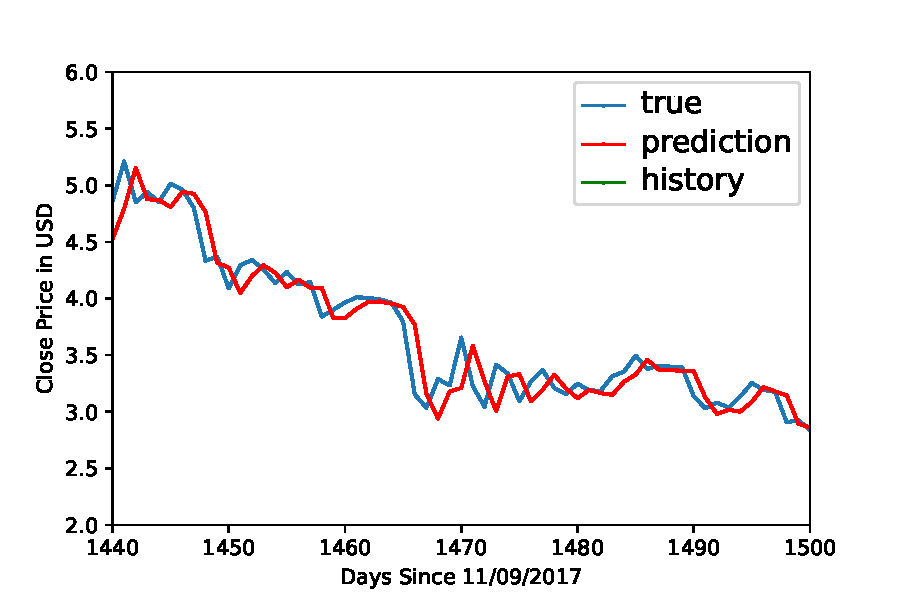
\includegraphics[width=\textwidth]{images/EOS-USD-epoch-100.pdf}
         \caption{100 Epochs}
         \label{fig:epochs-100}
     \end{subfigure}

\caption{Effect of EOS-USD prediction model based on the number of epochs completed.}
\label{fig:epoch}
\end{figure*}

The number of training epochs can affect the Root Mean Squared Error of the model, which details how close the prediction line is to the real, historical Close prices in United States Dollars (USD). As demonstrated in Table \ref{tab:epochvsrmse}, more epochs lessens the Root Mean Squared Error (but the change becomes negligible after 25 epochs).

Figure \ref{fig:epoch} also shows the impact that epochs have on accuracy. Figure \ref{fig:epoch} contains two lines: a blue line for the actual price of the EOS coin, and a red line for the model's prediction of the price. As the number of epochs increases, the prediction becomes more and more accurate to the actual price that the cryptocoin was valued at on the market. In Figure \ref{fig:epoch}, the green "history" line is not shown because the graph is zoomed in to the later prediction phase, where the historical price data becomes the blue line instead of green.

\begin{table}[htb]
\caption{Number of epochs compared with Root Mean Squared Error rounded to the nearest thousandth; all tests were run with EOS-USD as input.}
\label{tab:epochvsrmse}
\begin{tabular}{rl}
Epochs &   Root Mean Squared Error   \\
\hline
 5      & 0.523 USD              \\
 15     & 0.286 USD              \\
 25     & 0.260 USD              \\
 50     & 0.235 USD              \\
 100    & 0.229 USD              \\
\hline
\end{tabular}
\end{table}

Lastly, cryptocurrencies other than EOS such as Dogecoin, Ethereum, and Bitcoin can be analyzed as well. Figure \ref{fig:other} demonstrates the prediction models generated for these cryptocurrencies. Dogecoin presents a model with predictions that are more widely offset than the other coins, likely because most of the training period encompasses a period of relative inactivity (no high changes in price). 


\begin{figure*}[p]
\begin{minipage}{.05\textwidth}

\includegraphics[width=1.0\textwidth]{images/eos-usd.png}
\end{minipage}
\ \
\begin{minipage}{.4\textwidth}
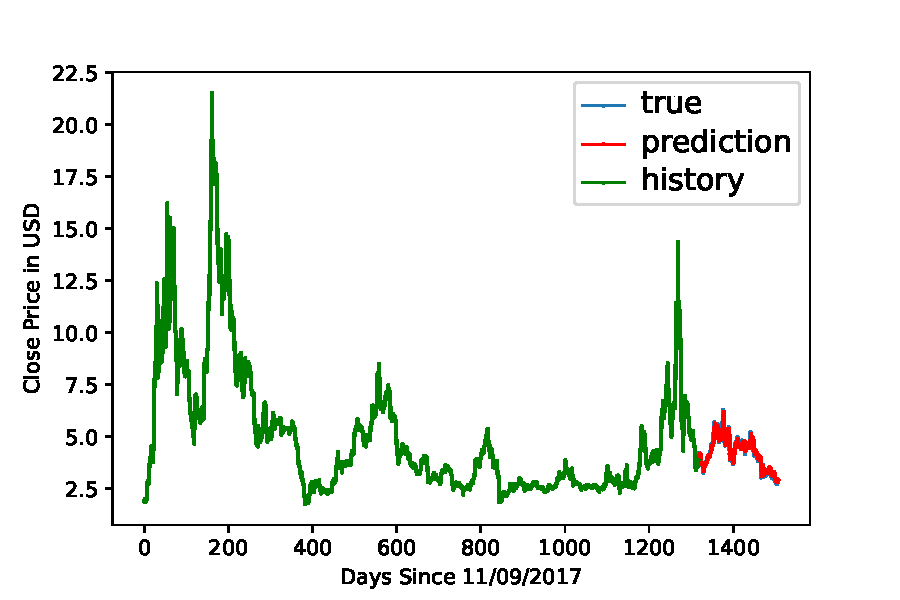
\includegraphics[width=1.0\textwidth]{images/EOS-USD-prediction-model.pdf}
\end{minipage}
\ \
\begin{minipage}{.4\textwidth}
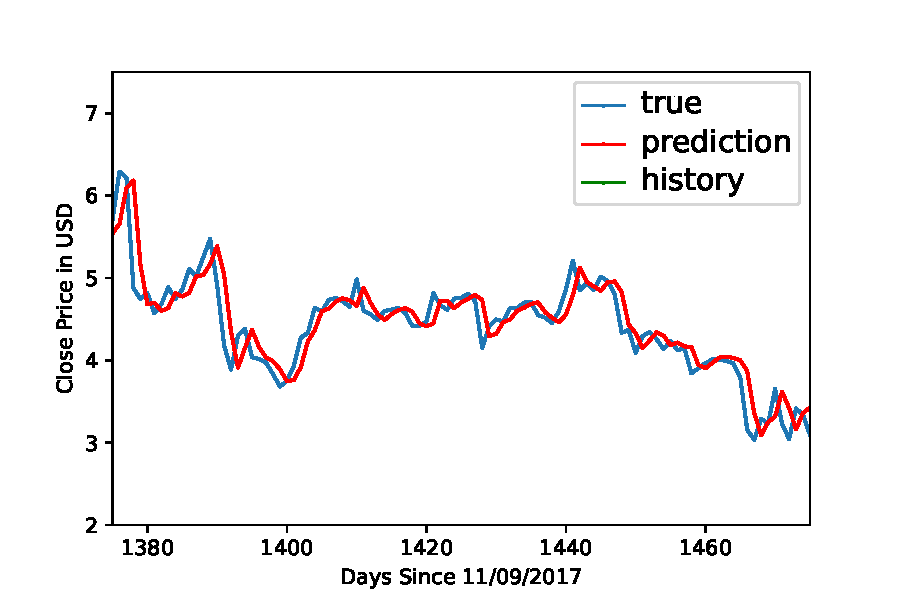
\includegraphics[width=1.0\textwidth]{images/EOS-USD-prediction-model-zoomed.pdf}
\end{minipage}

\begin{minipage}{.05\textwidth}

\includegraphics[width=1.0\textwidth]{images/doge-usd.png}
\end{minipage}
\ \
\begin{minipage}{.4\textwidth}
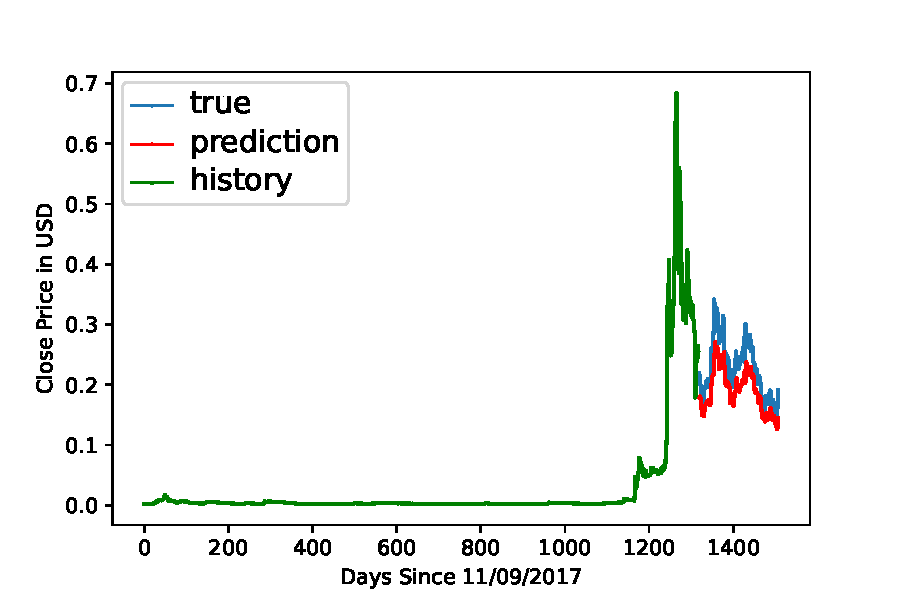
\includegraphics[width=1.0\textwidth]{images/DOGE-USD-prediction-model.pdf}
\end{minipage}
\ \
\begin{minipage}{.4\textwidth}
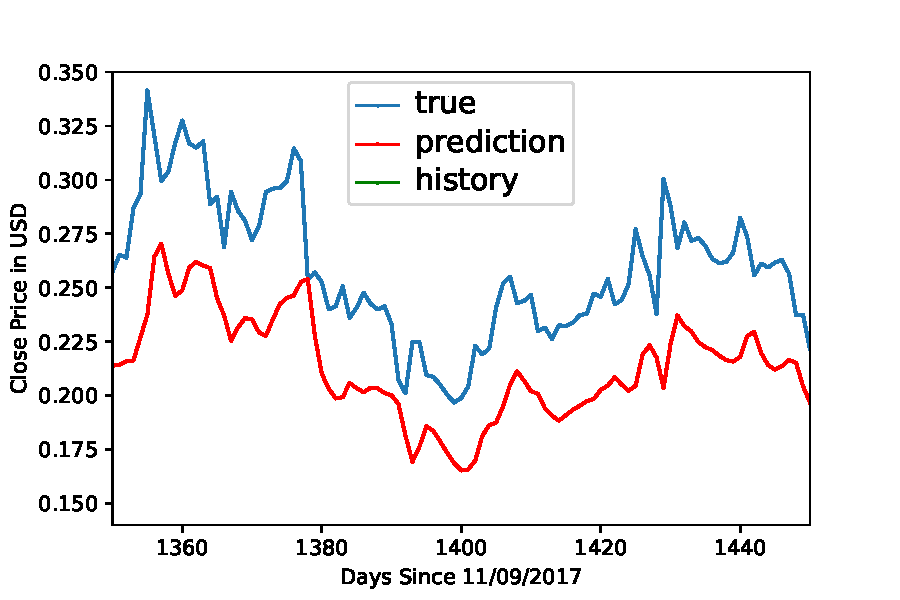
\includegraphics[width=1.0\textwidth]{images/DOGE-USD-prediction-model-zoomed.pdf}
\end{minipage}

\begin{minipage}{.05\textwidth}

\includegraphics[width=1.0\textwidth]{images/eth-usd.png}
\end{minipage}
\ \
\begin{minipage}{.4\textwidth}
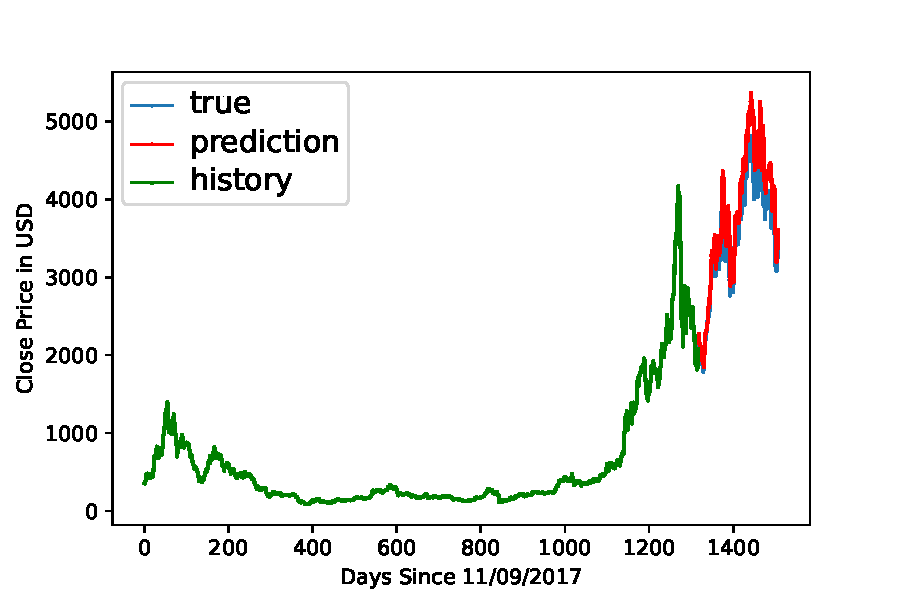
\includegraphics[width=1.0\textwidth]{images/ETH-USD-prediction-model.pdf}
\end{minipage}
\ \
\begin{minipage}{.4\textwidth}
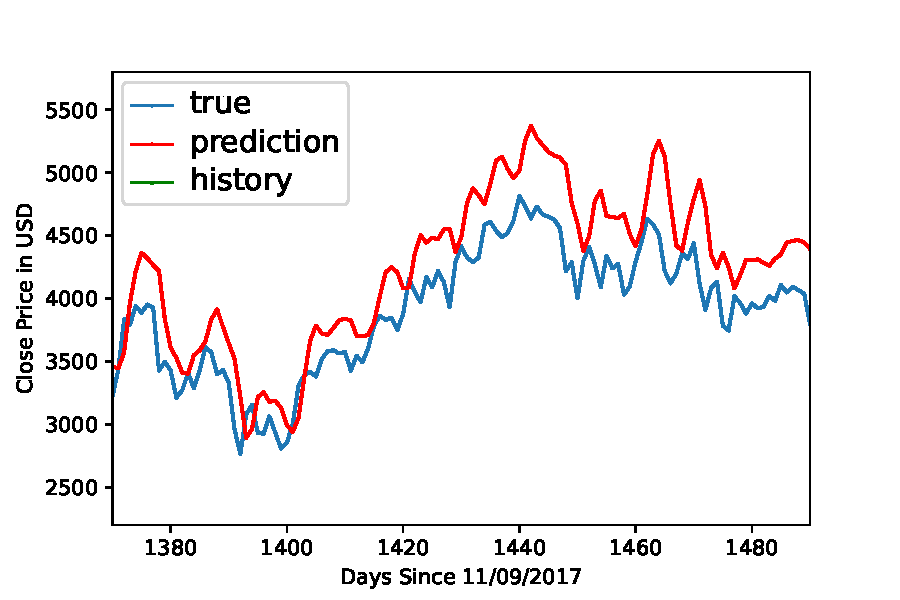
\includegraphics[width=1.0\textwidth]{images/ETH-USD-prediction-model-zoomed.pdf}
\end{minipage}

\begin{minipage}{.05\textwidth}

\includegraphics[width=1.0\textwidth]{images/btc-usd.png}
\end{minipage}
\ \
\begin{minipage}{.4\textwidth}
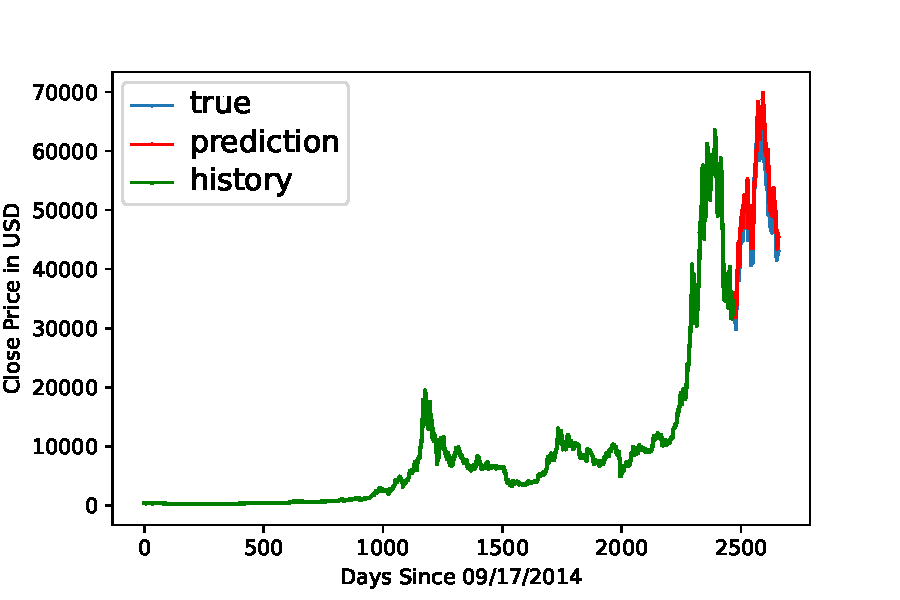
\includegraphics[width=1.0\textwidth]{images/BTC-USD-prediction-model.pdf}
\end{minipage}
\ \
\begin{minipage}{.4\textwidth}
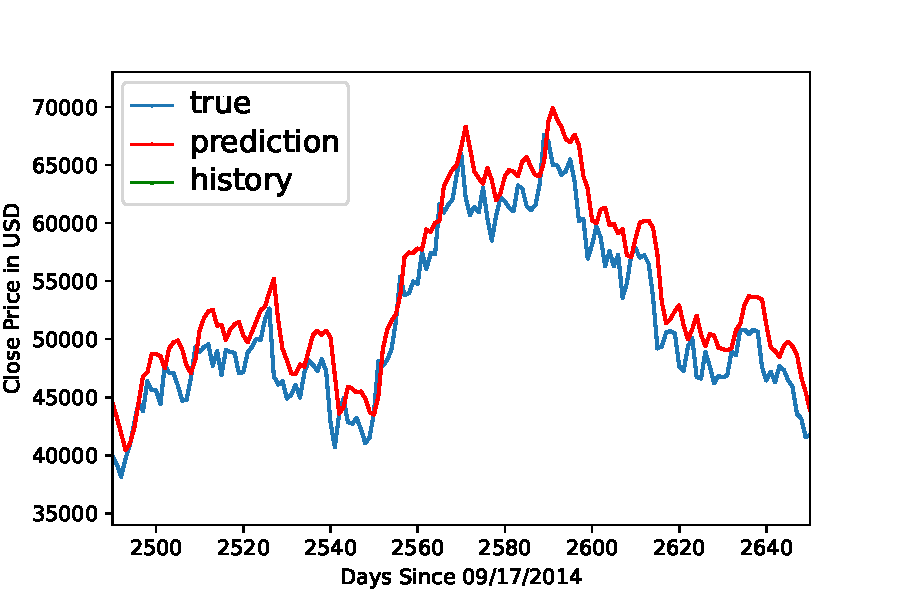
\includegraphics[width=1.0\textwidth]{images/BTC-USD-prediction-model-zoomed.pdf}
\end{minipage}

\caption{EOS, Dogecoin, Ethereum, and Bitcoin prediction models.}
\label{fig:other}
\end{figure*}


\section{Benchmark}

The benchmark is run within yfinance-lstm.ipynb located in project/code \cite{c13}. The program ran on a 64-bit Windows 10 Home Edition (21H1) computer with a Ryzen 5 3600 processor (3.6 GHz). It also has dual-channel 16 GB RAM clocked at 3200 MHz and a GTX 1660 Ventus XS OC graphics card. Table \ref{tab:resource} lists these specifications as well as the allocated computer memory during runtime and module versions. Table \ref{tab:second} shows that the amount of time it takes to train the 50 epochs for the LSTM is around 15 seconds, while the entire program execution takes around 16 seconds. A StopWatch module was used from the package cloudmesh-common \cite{c10} to precisely measure the training time.

In Table 3, the time column reports the length of the program phase in seconds. Training time and prediction time do not perfectly add up to overall time because the time it took to split data into train and test sets is not part of the training or prediction phases. Furthermore, the start times are similar because the entire program's cells were run consecutively.
 
\begin{table}[htb]
\caption{Benchmark details including the specifications and status of the computer at the time of program execution.}
\label{tab:resource}
\begin{tabular}{p{2cm}p{5cm}}
Attribute        & Value  \\
\hline
 cpu cores        & 6    \\
 cpu threads      & 12    \\
 cpu frequency    & 3600.0 MHz      \\
 mem.available    & 7.1 GiB \\
 mem.percent      & 55.3 \%  \\
 mem.total        & 16.0 GiB \\
 mem.used         & 8.8 GiB  \\
 python           & 3.9.5 (tags/v3.9.5:0a7dcbd, May  3 2021, 17:27:52) [MSC v.1928 64 bit (AMD64)]  \\
 python.pip       & 21.1.3   \\
 python.version   & 3.9.5 \\
 uname.processor  & AMD64 Family 23 Model 113 Stepping 0, AuthenticAMD   \\
 uname.system     & Windows \\
 uname.version    & 10.0.19043 \\
 \hline
 \end{tabular}
 \end{table}


\begin{table}[htb]
\caption{Benchmark output which reports the execution time of overall program, training phase, and prediction phase.}
\label{tab:second}
\begin{tabular}{lrrll}
Name            &   Time   & Start               & OS Version \\
\hline
 Overall time    & 16.589 s & 2021-07-26 18:39:57 & Windows  10.0.19043, SP0 \\
Training time   & 15.186 s & 2021-07-26 18:39:58 & Windows 10.0.19043, SP0 \\
 Prediction time &  0.227 s & 2021-07-26 18:40:13 & Windows 10.0.19043, SP0 \\
 \hline
 \end{tabular}
 \end{table}
 
\section{Conclusion}

At first glance, the results look promising as the predictions have minimal deviation from the true values (as seen in Figure \ref{fig:zoomed}). However, upon closer look, the values lag by one day, which is a sign that they are only viewing the previous day and mimicking those values. Furthermore, the model cannot go several days or years into the future because there is no data to run on, such as opening price or volume. The experiment is further confounded by the nature of stock prices: they follow random walk theory, which means that the nature in which they move follows a random walk: the changes in price do not necessarily happen as a result of previous changes. Thus, this nature of stocks contradicts the very architecture of this experiment because long short-term memory assumes that the values have an effect on one another.

For future research, a program can scrape tweets from influencers' Twitter pages so that a model can guess whether public discussion of a cryptocurrency is favorable or unfavorable (and whether the price will increase as a result).


\begin{acks}
Thank you to Florida A\&M University for graciously funding this scientific excursion and the Miami Dade College School of Science for this research opportunity. Work supported by Gregor von Laszewski was supported by the NSF Grant \#1829704: CyberTraining: CIC: CyberTraining for Students and Technologies from Generation Z.
Work conducted by members of FAMU and Jacques Fleischer was supported, in part, by NSF Grant called Florida Georgia Louis Stokes Alliance for Minority Participation, with the subaward FAMU C-5083.
\end{acks}


\bibliographystyle{ACM-Reference-Format}
\bibliography{all}


\appendix

\section{Additional Material}

The following additional material is available:

\begin{description}

\item[Online Description] \cite{c14}

\item[Install documentation] \cite{c12}

\item[Python Notebook] yfinance-lstm.ipynb \cite{c13}

\item[Presentations] 
Presentations of this work were given at the
2021 FAMU-FGLSAMP Data Science and AI Research Experience for Undergraduates Presentation \cite{c15}
and as poster in the Miami Dade College School of Science 10th Annual STEM Research Symposium 2021 Poster \cite{c16}.

\end{description}


\bibliographystyle{ACM-Reference-Format}
\bibliography{paper-blockchain}


\appendix

\section{Additional Material}

The following additional material is available:

\begin{description}

\item[Online Description] \cite{c14}

\item[Install documentation] \cite{c12}

\item[Python Notebook] yfinance-lstm.ipynb \cite{c13}

\item[Presentations] 
Presentations of this work were given at the
2021 FAMU-FGLSAMP Data Science and AI Research Experience for Undergraduates Presentation \cite{c15}
and as poster in the Miami Dade College School of Science 10th Annual STEM Research Symposium 2021 Poster \cite{c16}.

\end{description}

\end{document}
\endinput
%%%%%%%%%%%%%%%%%%%%%%%%%%%%%%%%%%%%%%%%%%%%%%%%%%%%%%%%%%%%%%

